\documentclass[conference, a4paper]{IEEEtran}

% =========================================================
% PACKAGES
% =========================================================
\usepackage[T1]{fontenc}
\usepackage{cite}
\usepackage{amsmath,amssymb}
\usepackage{graphicx}
\usepackage{booktabs}
\usepackage{array}
\usepackage{url}
\usepackage{microtype}
\usepackage{listings}
\usepackage[section]{placeins}
\usepackage{tikz}
\usetikzlibrary{arrows.meta,positioning,shapes.geometric,fit,backgrounds}
\usepackage{caption}
\usepackage{multirow}
\captionsetup{font=small,skip=3pt}
\renewcommand{\arraystretch}{0.92}
\setlength{\textfloatsep}{6pt plus 2pt minus 2pt}
\setlength{\floatsep}{5pt plus 2pt minus 2pt}
\setlength{\intextsep}{6pt plus 2pt minus 2pt}

% =========================================================
% TITLE
% =========================================================
\title{
Verification-Guided Q-Learning for Web Vulnerability Testing:
An Empirical Evaluation of Discovery Efficiency
}

\author{
\IEEEauthorblockN{Kevin Imanuel Setiawan}
\IEEEauthorblockA{
Program Studi Teknologi Informasi, Fakultas Informatika\\
Telkom University Surabaya\\
Surabaya, Indonesia
}
}
\begin{document}

\maketitle

% =========================================================
% ABSTRACT & KEYWORDS
% =========================================================
\begin{abstract}
Automated web vulnerability testing can produce numerous
candidate findings, yet unusual application responses do not
necessarily indicate exploitable weaknesses. This study
evaluates a verification-guided Q-Learning prototype that
selects endpoint--payload actions against OWASP Juice Shop.
The agent observes HTTP responses, derives discrete state
features, and incorporates verification outcomes into reward
assignment. Its configured action space contains 120
endpoint--payload combinations, formed from eight endpoints
and 15 payloads per endpoint. Across five seeds, Q-Learning
verified a mean of 12.8 actions (SD 1.10; range 11--14) and
found all 14 reference actions in one run. A random policy found
all 14 in five runs, with mean full-coverage episode 308.4; a
fixed-order scan found all 14 by episode 66 in one run. A
Q-Learning ablation without verification-guided reward found a
mean of 13.0 actions across five seeds. These comparisons use
the same curated reference and verification procedure, so they
do not establish generalization or independent detector accuracy.
A separate detector benchmark reported recall 0.929 and F1-score
0.963 on 74 labelled actions; 46 unknown cases were excluded.
The results provide no evidence that Q-Learning improves
discovery efficiency in this fixed, source-informed action space.

\noindent\textit{Keywords}---Automated penetration testing, reinforcement learning,
Q-Learning, web vulnerability testing, vulnerability
verification, OWASP Juice Shop
\end{abstract}
% =========================================================
% 1. INTRODUCTION
% =========================================================
\section{Introduction}

Web applications expose user input to numerous interfaces,
endpoints, and server-side components, and mistakes in how that
input is handled or processed can introduce security weaknesses.
Automated security testing helps surface such weaknesses by
submitting test inputs and inspecting the resulting application
behavior. An unusual response is not, by itself, sufficient
evidence that a weakness can be exploited: error messages,
changes in response length, and other observable differences can
also arise during normal operation.

Reinforcement learning (RL) provides a framework for sequential
decision-making under feedback from an environment: an agent
selects an action, observes the consequence, and updates its
policy from the reward received. Q-Learning estimates the
expected return of state--action pairs from observed transitions
\cite{sutton2018}.

Learning-based approaches to security testing have been explored
in prior work. SQIRL applies reinforcement learning to grey-box
SQL injection detection \cite{sqirl2023}, and other studies have
investigated deep reinforcement learning for vulnerability
exploitation and autonomous penetration testing
\cite{almajali2024,li2025}. A recent survey traces the development
of reinforcement-learning approaches to automated penetration
testing and discusses open challenges \cite{rlreview2026}, and a
comparative study of autonomous penetration-testing agents reports
that their effectiveness depends heavily on the testing
environment, the action design, and the evaluation procedure
\cite{sok2024}.

A central problem in automated testing is deciding when an
observation should count as a finding. A response anomaly may
point to a candidate weakness, but confirming it requires evidence
specific to the testing category rather than the anomaly alone.
This study evaluates a verification-guided Q-Learning prototype
built around that separation: candidate signals are kept distinct
from actions that satisfy an explicit verification procedure.

The study makes three contributions:

\begin{itemize}
    \item it presents a Q-Learning workflow in which verification
    evidence, rather than the raw response anomaly, drives reward
    assignment;

    \item it compares Q-Learning against random and fixed-order
    action selection and reports a reward-verification ablation,
    all within the same configured Juice Shop action space and
    request budget; and

    \item it evaluates the prototype's detector against a labelled
    reference set using recall and F1-score, while explicitly
    reporting that the labels are not independent of the
    prototype's own verification evidence.
\end{itemize}

The scope is limited to the configured application, the
configured endpoint--payload combinations, and the experimental
procedures described below; the results are not intended to
establish performance on arbitrary web applications. Endpoint and
payload selection relied on source-informed prior knowledge of the
target. Under a matched primary-action budget, random and
fixed-order selection recovered the curated reference findings
earlier than Q-Learning, so the results reported here do not
support an efficiency benefit attributable to Q-Learning in this
setting.

% =========================================================
% 2. RELATED WORK
% =========================================================
\section{Related Work}

Reinforcement learning has been applied to security testing and
vulnerability discovery in several forms. SQIRL targets grey-box
SQL injection detection \cite{sqirl2023}; other work applies deep
RL to vulnerability exploitation \cite{almajali2024}, partially
observable testing agents \cite{li2025}, and larger network
environments \cite{ghanem2023}. Survey and comparative studies
consistently note that reported results depend on the target
application, the action-space design, and the evaluation protocol
\cite{rlreview2026,sok2024} -- a dependency this study treats as a
methodological constraint rather than a limitation to engineer away.

The OWASP Web Security Testing Guide offers structured guidance for
web security assessments \cite{owaspwstg}. This study follows its
principle that an HTTP anomaly is only a candidate signal:
SQL-injection and file-disclosure candidates undergo control checks,
while cross-site scripting (XSS) candidates are confirmed through a
browser execution check built with Playwright \cite{playwright}.
These checks define the scope of the prototype's claims; they do
not constitute an independently audited oracle, nor do they
establish generalization beyond the configured target.

\section{Methodology}

\subsection{Experimental Environment}

Experiments used OWASP Juice Shop version 20.2.0 running locally.
Juice Shop is an intentionally insecure web application built for
security education and testing \cite{juiceshop}.

The target base URL was \url{http://localhost:3000}, and the HTTP
client enforced a 10-second request timeout. To reproduce the
setup with the repository's local Juice Shop 20.2.0 source tree,
run \texttt{cd juice-shop; npm start}; the application then becomes
reachable at the target base URL. Each trial began with eight
benign endpoint probes that established per-endpoint
response-length baselines before training started.

All reported experiments ran on the local Juice Shop 20.2.0 source
tree under Windows, with Node.js v24.22.1. The server was started
with \texttt{node build/app.js}, the same command invoked by the
project's \texttt{npm start} script. Because the SQLite database is
reinitialized by the application on every restart, each trial began
from a freshly populated instance. The launch configuration used
for an earlier, unreported single-seed run was not recorded; all
results reported below come from the setup described here.

The prototype operates over a configured set of eight endpoints and
15 payloads per endpoint. At each step the Q-Learning agent selects
an endpoint--payload action, submits the corresponding request,
observes the resulting HTTP response, and updates its
state--action value estimate according to the assigned reward.

These results describe one reported configuration; different
application versions, endpoint sets, payload sets, or verification
rules may produce different outcomes.

\subsection{HTTP API and Endpoint Coverage}

The target is reached through HTTP routes exposed by Juice Shop,
covering REST API routes and the \texttt{/ftp/} file-serving route.
For each selected action, the client places the payload in the
route's configured query parameter, appends it to the route when
the parameter is path-based, or embeds it in a JSON body for POST
and PUT requests. Response status, body length, content type, and
response time together form the observations used to construct the
state. Table~\ref{tab:api-endpoints} lists the eight routes used by
the agent.

\begin{table}[!t]
\caption{HTTP Routes Used in the Experiment}
\label{tab:api-endpoints}
\centering
\footnotesize
\setlength{\tabcolsep}{3pt}
\begin{tabular}{c p{0.41\columnwidth} p{0.43\columnwidth}}
\toprule
\textbf{Idx.} & \textbf{Method and route} & \textbf{Role in the experiment}\\
\midrule
0 & GET \url{/rest/products/search?q=} & Product search; SQLi and search-page XSS checks\\
1 & GET \url{/ftp/} + path & File-serving route; path and extension-bypass checks\\
2 & GET \url{/rest/products/1/reviews?id=} & Review retrieval; plain-surface control\\
3 & GET \url{/rest/track-order/} + path & Order tracking; browser-based XSS checks on the result page\\
4 & POST \url{/rest/user/login} & Login request with a JSON body; SQLi checks\\
5 & PUT \url{/rest/products/1/reviews} & Review submission with a JSON body; plain-surface control\\
6 & POST \url{/api/Feedbacks} & Feedback JSON body; requires CAPTCHA fields\\
7 & GET \url{/api/Challenges?q=} & Challenge API; plain-surface control\\
\bottomrule
\end{tabular}
\end{table}
\setlength{\tabcolsep}{6pt}

Endpoint selection drew on inspection of the Juice Shop 20.2.0
source and is therefore part of the human prior built into the
experiment. The search route (index 0) and the login route
(index 4) were included because their inputs reach SQL-related
handlers; the file-serving route (index 1) was included for path
and extension-filter checks; and the track-order route (index 3)
was included because its identifier is rendered on a browser page.
Review retrieval (index 2), review submission (index 5), feedback
submission (index 6), and the challenge API (index 7) serve as
contrasting or control surfaces and were not selected through any
autonomous endpoint-discovery process. The experiment therefore
evaluates action selection within a researcher-defined attack
surface rather than discovery of an unknown application's
endpoints.

The feedback route requires an additional GET request to
\url{/rest/captcha}; the returned answer and identifier are then
included with the feedback JSON body, together with the configured
defaults \texttt{rating=1} and \texttt{UserId=1}. Before training
begins, the prototype sends a benign \texttt{hello} probe to each
of the eight routes to establish endpoint-specific response
baselines. The two XSS-capable routes are additionally checked
through their corresponding Juice Shop single-page application
(SPA) pages, since an HTTP response that merely contains a vector
does not show that a browser executed it. The configured
\texttt{sql}, \texttt{file}, and \texttt{plain} surface labels
restrict which detector checks apply to each route; they are
source-informed metadata about possible input sinks rather than
preassigned vulnerability findings, and every candidate must still
pass the verification workflow described in
Section~\ref{sec:verification}.

\subsection{Action Space}

Let $\mathcal{E}$ denote the configured endpoint set and
$\mathcal{P}$ the configured payload set. The action space is

\begin{equation}
\mathcal{A} = \mathcal{E} \times \mathcal{P}.
\label{eq:actionspace}
\end{equation}

With eight endpoints and 15 payloads per endpoint, the number of
configured endpoint--payload combinations is

\begin{equation}
|\mathcal{A}| = |\mathcal{E}| \times |\mathcal{P}|
= 8 \times 15 = 120.
\label{eq:actioncount}
\end{equation}

Table~\ref{tab:payloads} lists the 15 payload templates. Each
template is paired with each of the eight endpoint configurations;
the client places it in the configured query parameter, path, or
JSON body. The long-input probe consists of 1,628 ASCII \texttt{A}
characters. This Cartesian product is fixed before training
begins, and does not change during a run.

\begin{table*}[!t]
\caption{Configured Payload Templates}
\label{tab:payloads}
\centering
\scriptsize
\begin{tabular}{p{0.20\textwidth}p{0.12\textwidth}p{0.63\textwidth}}
\toprule
\textbf{Name} & \textbf{Class} & \textbf{Payload}\\
\midrule
\texttt{sqli\_tautology} & SQLi & \lstinline|' OR '1'='1|\\
\texttt{sqli\_comment} & SQLi & \lstinline|apple'--|\\
\texttt{sqli\_union} & SQLi & \lstinline|' UNION SELECT NULL--|\\
\texttt{sqli\_time} & SQLi & \lstinline|' OR SLEEP(5)--|\\
\texttt{sqli\_wildcard} & SQLi & \lstinline|%s%s%s%s%s%s%s%s|\\
\texttt{sqli\_login} & SQLi & \lstinline|{"email":"admin@juice-sh.op' OR '1'='1","password":"a"}|\\
\texttt{xss\_img} & XSS & \lstinline|<img src=x onerror=alert(document.domain)>|\\
\texttt{xss\_script} & XSS & \lstinline|<script>alert(document.domain)</script>|\\
\texttt{xss\_svg} & XSS & \lstinline|<svg onload=alert(1)>|\\
\texttt{xss\_review} & XSS & \lstinline|{"message":"<img src=x onerror=alert(document.domain)>","author":"rlpoc"}|\\
\texttt{lfi\_poison\_null} & File & \lstinline|package.json.bak%2500.md|\\
\texttt{lfi\_coupons} & File & \lstinline|coupons_2013.md.bak%2500.md|\\
\texttt{lfi\_wap\_rules} & File & \lstinline|suspicious_errors.yml%2500.pdf|\\
\texttt{fuzz\_long} & Fuzzing & \texttt{A} repeated 1,628 times\\
\texttt{fuzz\_null} & Fuzzing & \lstinline|admin%00|\\
\bottomrule
\end{tabular}
\end{table*}

An action corresponds to submitting one configured template to one
selected endpoint; the resulting response is processed to
construct the next state. Episode-to-full-coverage figures
reported in Section~\ref{sec:results} are averaged only over trials
that found all 14 reference actions. Mean total request counts
include the eight benign baseline probes together with the actual
control and browser verification requests; primary-action budgets
are matched across methods, while total HTTP interactions vary
slightly across runs because verification overhead depends on
which candidates are raised. Payload and surface selection rely on
known Juice Shop behavior; this prior constrains the scope of the
experiment and must not be read as evidence of fully autonomous
vulnerability discovery.

\subsection{State Representation}

The prototype represents each observation using eight discrete
features:

\begin{equation}
\begin{split}
s_t = (&\text{status\_cat},
\text{length\_cat},
\text{err\_flag},
\text{refl\_flag},\\
&\text{vuln\_ind},
\text{ep\_idx},
\text{resp\_time\_cat},
\text{content\_cat}).
\end{split}
\label{eq:state}
\end{equation}

These features encode, respectively, the HTTP status category,
the response-length category, an error flag, a reflection flag, a
vulnerability indicator, the endpoint index, a response-time
category, and a content-type category.

Response-length deviation is measured against the configured
per-endpoint baseline; a deviation greater than 15\% is treated as
a significant change. Response time is classified as fast below
0.5 seconds, medium between 0.5 and 2.0 seconds, and slow above
2.0 seconds.

This representation reduces selected HTTP response characteristics
to a small set of discrete features. Because the agent's next
action is conditioned only on this state summary -- not on any
explicit model of the target's internal or session state -- its
state transition should be read as scheduling context for the next
probe rather than as a representation of application behavior; this
point is revisited in Section~\ref{sec:protocol}. Consequently, the
representation's coverage of real application behavior is bounded
by the features and thresholds implemented in the prototype.

\subsection{Q-Learning Update}

The agent updates the value of a state--action pair from the
observed reward and the maximum estimated value of the next state:

\begin{equation}
\footnotesize
Q(s_t,a_t) \leftarrow Q(s_t,a_t) + \alpha \big[ r_t + \gamma \max_{a'} Q(s_{t+1},a') - Q(s_t,a_t) \big],
\label{eq:ql}
\end{equation}

where $s_t$ is the current state, $a_t$ is the selected action,
$r_t$ is the observed reward, $s_{t+1}$ is the next state, $\alpha$
is the learning rate, and $\gamma$ is the discount factor
\cite{sutton2018}.

The reported configuration uses $\alpha=0.1$ and $\gamma=0.9$. An
$\epsilon$-greedy policy balances exploration and exploitation:
$\epsilon$ starts at 1.0, is multiplied by 0.90 after every
episode, and is floored at 0.1. Under this schedule,
$\epsilon_n=\max(0.1,0.9^{n-1})$ for episode $n$, so the floor is
reached at episode 23, after 22 decay updates; if high exploration
is defined as $\epsilon\geq0.5$, only the first seven episodes meet
that threshold. This decay rate was a configured design choice
rather than the outcome of a sensitivity study, so each Q-Learning
run spends nearly all of its 1,585-episode budget at the
exploration floor -- a point that bears directly on the comparative
results in Section~\ref{sec:results}. Only actions already verified
as vulnerable are masked from future selection; unsuccessful
actions remain selectable throughout, and no run terminates early.

\subsection{Comparative Experimental Protocol}
\label{sec:protocol}

Every method received an identical budget of 1,585 primary
endpoint--payload episodes. Q-Learning and uniform random selection
were each run with seeds 42--46; the fixed-order baseline visited
action indices in ascending order, wrapping after the final index
and skipping only actions already verified, and was run once since
its selection order is deterministic. All policies shared the same
verified-action mask. A verification-reward ablation, also run with
seeds 42--46, retained the full verifier for logging and action
masking but supplied the Q-Learning update with the
pre-verification analyzer reward, so a control or browser verdict
could not increase the credited reward. Reward sensitivity was
evaluated separately with three paired seeds (42--44): a lower
setting of $+25/+5/-1/-5$ and a higher setting of $+100/+20/-1/-5$
for verified/anomaly/normal/error outcomes, respectively, with the
length bonus held constant. Every trial used a freshly restarted
Juice Shop instance.

The primary-action budget was identical across methods, while total
HTTP interactions varied from 1,629 to 1,640 because the number of
control and browser-verification requests depends on which actions
are raised as candidates; both counts are reported in
Table~\ref{tab:strategy-results}, and none of the runs caps total
interactions once verification overhead is included.

At each episode the selected request is conditioned on the state
summary produced by the preceding request. The target's application
or session state is not modeled explicitly, and requests to
different endpoints are not treated as steps in an exploit chain, so
$s_{t+1}$ functions as observation-derived scheduling context for
the next probe rather than evidence of a stateful application
transition. This formulation permits response-conditioned action
selection, but given the finite action space and the absence of a
matched exhaustive-search baseline, it does not support attributing
any discovery-efficiency difference to the Q-Learning update itself.

\subsection{Verification-Guided Reward Assignment}
\label{sec:verification}

The base rewards are $+50$ for a verified finding, $+10$ for an
unverified anomaly, $-1$ for a normal response, and $-5$ for an
attack-request connection failure or timeout, with a
response-length bonus of $+0$, $+0$, $+5$, or $+10$ added by length
category. SQL-injection and file-disclosure candidates receive a
benign \texttt{hello} control and, when distinct from the attack
payload, a neutralized-payload control; a candidate is verified only
if neither control reproduces the same response class as the attack
request. For XSS, headless Chromium loads the matching SPA page with
an instrumented vector, and verification requires that the DOM
canary execute while a distinct neutralized control does not -- HTTP
reflection alone is insufficient. A failed attack request receives
$-5$; a failed control instead makes the candidate inconclusive and
unverified, without the $-5$ penalty, after which the base reward is
$+10$ only if anomaly flags remain set and $-1$ otherwise, with the
length bonus still applied.

On SQL-surface endpoints, candidates are raised by a database-error
signature co-occurring with an HTTP error, or by a successful
SQL-like request whose response length changes by at least 15\%
from baseline; the wildcard payload follows a corresponding
successful-response rule. On the file surface, a directory listing
or a bare size change is not treated as disclosure on its own;
evidence requires either known content markers (such as Juice Shop
package metadata) or a successful \texttt{\%2500} extension bypass
serving a type outside Markdown, plain text, or PDF, probing
\texttt{package.json.bak}, \texttt{coupons\_2013.md.bak}, and
\texttt{suspicious\_errors.yml}. The retained logs omit response
bodies and content types, so individual SQLi and file-disclosure
evidence cannot be reconstructed retrospectively (Section~\ref{sec:limitations}).

These reward values are design choices rather than optimized
parameters; the three-seed sensitivity comparison is reported in
Section~\ref{sec:reward-sensitivity}.

\subsection{Evaluation Metrics}

The reference-set evaluation uses true positives (TP), false
positives (FP), false negatives (FN), and true negatives (TN).
Recall measures the share of labelled vulnerable actions detected,
and F1-score combines recall with precision; cases marked unknown
are excluded, so the reported values describe only the labelled
subset.

\begin{equation}
\mathrm{Recall} = \frac{TP}{TP+FN}.
\label{eq:recall}
\end{equation}

\begin{equation}
\mathrm{F1} =
2\frac{\mathrm{Precision}\times\mathrm{Recall}}
{\mathrm{Precision}+\mathrm{Recall}}.
\label{eq:f1}
\end{equation}

% =========================================================
% 4. RESULTS AND DISCUSSION
% =========================================================
\section{Results and Discussion}
\label{sec:results}

\subsection{System Workflow}

Fig.~\ref{fig:combined}(a) summarizes how one episode moves from
action selection through verification to the Q-table update
described in Sections~\ref{sec:protocol}
and~\ref{sec:verification}; Fig.~\ref{fig:combined}(b), discussed in
Section~\ref{sec:comparative}, plots verified-action discovery
against episode for all four compared methods.

\begin{figure*}[!t]
\centering
\begin{minipage}{0.46\textwidth}
\centering
\resizebox{0.92\textwidth}{!}{%
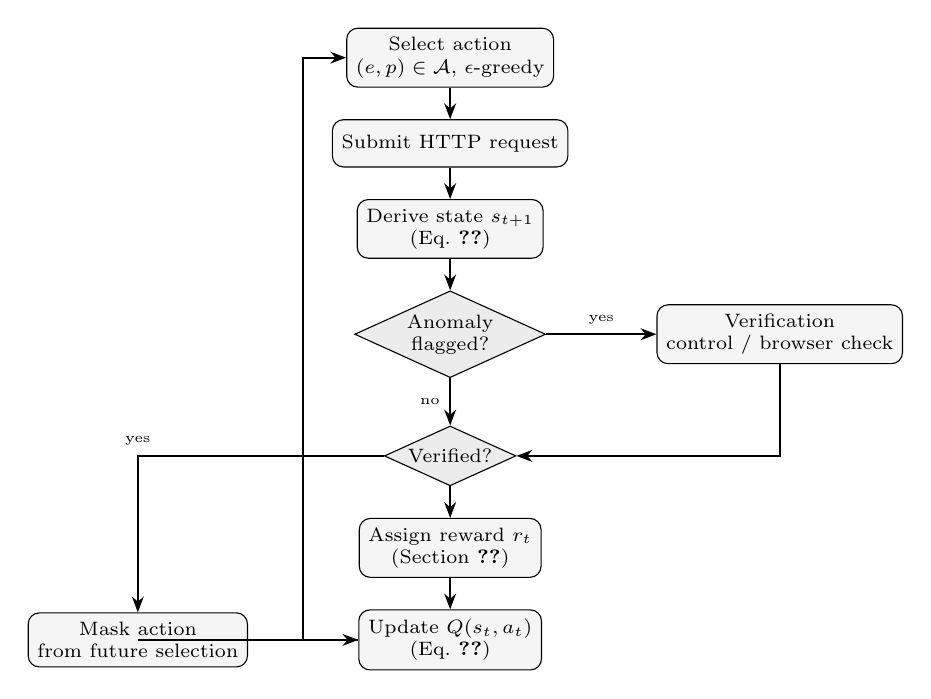
\begin{tikzpicture}[
  node distance=4mm and 5mm,
  box/.style={draw, rounded corners, align=center, minimum height=6mm,
    minimum width=21mm, font=\scriptsize, fill=gray!8},
  decision/.style={draw, diamond, align=center, font=\scriptsize,
    aspect=2.2, inner sep=1pt, fill=gray!15},
  arr/.style={-{Stealth[length=2mm]}, thick}
]
\node[box] (select) {Select action\\$(e,p)\in\mathcal{A}$, $\epsilon$-greedy};
\node[box, below=of select] (request) {Submit HTTP request};
\node[box, below=of request] (state) {Derive state $s_{t+1}$\\(Eq.~\ref{eq:state})};
\node[decision, below=of state] (anomaly) {Anomaly\\flagged?};
\node[box, right=of anomaly, xshift=9mm] (verify) {Verification\\control / browser check};
\node[decision, below=of anomaly, yshift=-2mm] (verified) {Verified?};
\node[box, below=of verified] (reward) {Assign reward $r_t$\\(Section~\ref{sec:verification})};
\node[box, below=of reward] (update) {Update $Q(s_t,a_t)$\\(Eq.~\ref{eq:ql})};
\node[box, left=of update, xshift=-9mm] (mask) {Mask action\\from future selection};

\draw[arr] (select) -- (request);
\draw[arr] (request) -- (state);
\draw[arr] (state) -- (anomaly);
\draw[arr] (anomaly) -- node[above,font=\tiny]{yes} (verify);
\draw[arr] (verify) |- (verified);
\draw[arr] (anomaly) -- node[left,font=\tiny]{no} (verified);
\draw[arr] (verified) -- (reward);
\draw[arr] (reward) -- (update);
\draw[arr] (verified) -| node[above,font=\tiny]{yes} (mask);
\draw[arr] (mask) |- (update);
\draw[arr] (update.west) -- ++(-7mm,0) |- (select.west);
\end{tikzpicture}%
}
\centerline{\scriptsize (a) Per-episode workflow}
\end{minipage}
\hfill
\begin{minipage}{0.50\textwidth}
\centering
\resizebox{0.96\textwidth}{!}{%
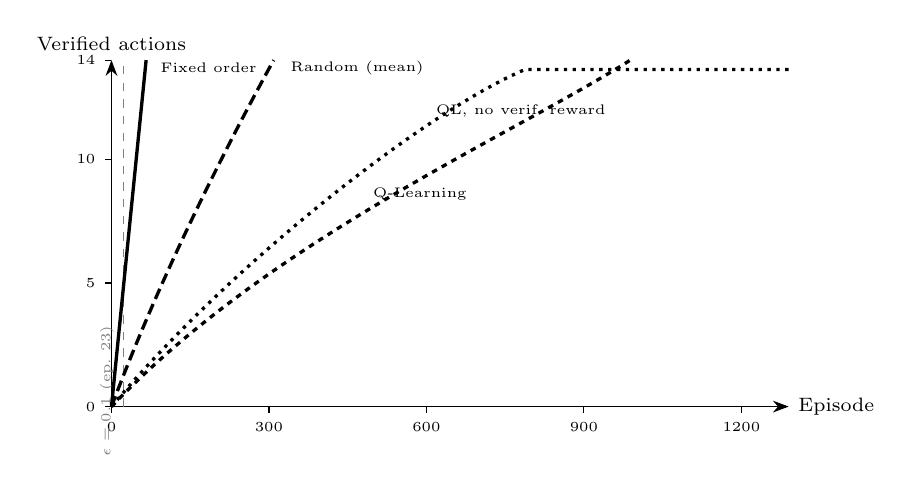
\begin{tikzpicture}
\begin{scope}
\draw[-{Stealth[length=2mm]}] (0,0) -- (8.6,0) node[right,font=\scriptsize]{Episode};
\draw[-{Stealth[length=2mm]}] (0,0) -- (0,4.4) node[above,font=\scriptsize]{Verified actions};
\foreach \x/\lbl in {0/0, 2/300, 4/600, 6/900, 8/1200} {
  \draw (\x,0) -- (\x,-0.08) node[below,font=\tiny]{\lbl};
}
\foreach \y/\lbl in {0/0, 1.57/5, 3.14/10, 4.4/14} {
  \draw (0,\y) -- (-0.08,\y) node[left,font=\tiny]{\lbl};
}
\draw[dashed, gray] (0.153,0) -- (0.153,4.4);
\node[font=\tiny, gray, rotate=90, anchor=south] at (0.153,0.2) {$\epsilon=0.1$ (ep.\ 23)};

% Fixed order: steep rise to 14 by episode 66
\draw[very thick] (0,0) -- (0.44,4.4);
\node[font=\tiny, anchor=west] at (0.5,4.3) {Fixed order};

% Random: mean full coverage at 308.4
\draw[very thick, dash pattern=on 4pt off 2pt]
  (0,0) .. controls (0.6,1.6) and (1.4,3.2) .. (2.06,4.4);
\node[font=\tiny, anchor=west] at (2.15,4.3) {Random (mean)};

% QL without verification reward: mean to 989
\draw[very thick, dash pattern=on 2pt off 2pt]
  (0,0) .. controls (2,2.1) and (5,3.4) .. (6.59,4.4);
\node[font=\tiny, anchor=west] at (4.0,3.75) {QL, no verif.\ reward};

% Q-Learning: mean to 787, plateau near 12.8
\draw[very thick, dotted]
  (0,0) .. controls (1.5,1.8) and (4,3.75) .. (5.25,4.28)
  -- (8.6,4.28);
\node[font=\tiny, anchor=west] at (3.2,2.7) {Q-Learning};
\end{scope}
\end{tikzpicture}%
}
\centerline{\scriptsize (b) Schematic discovery curves}
\end{minipage}
\caption{(a) Per-episode workflow: action selection, request
submission, state derivation, verification (control checks for
SQLi/file candidates, browser checks for XSS candidates), reward
assignment, and the Q-table update; verified actions are masked
from future selection. (b) Verified-action count against episode
for all four compared methods, positioned from the reported mean
episode-to-all-14 values and final counts in
Table~\ref{tab:strategy-results} (illustrative interpolation
between episodes, not raw per-episode log data); the dashed
vertical line marks the episode at which $\epsilon$ reaches its
floor of 0.1.}
\label{fig:combined}
\end{figure*}

\subsection{Comparative Results}
\label{sec:comparative}

Table~\ref{tab:strategy-results} summarizes all 22 trials; every
trial used 1,585 primary endpoint--payload episodes against the
same 14-action reference set used in the detector benchmark, which
is itself drawn from the curated labels rather than an independent
oracle. Q-Learning verified a mean of 12.8 actions (SD 1.10; range
11--14), with only one of five seeds reaching all 14. Uniform
random selection reached all 14 in every seed, and the fixed-order
scan reached all 14 by episode 66 in its single deterministic run.
The random baseline's mean episode for full coverage was 308.4
(range 217--440). Fig.~\ref{fig:combined}(b) plots verified-action
count against episode for all four methods. Taken together, these
results give no evidence that Q-Learning improves discovery
efficiency within this fixed action space.

\begin{table*}[!t]
\caption{Matched Primary-Action Budget Comparison}
\label{tab:strategy-results}
\centering
\scriptsize
\begin{tabular}{p{0.20\textwidth}c p{0.28\textwidth}c c p{0.17\textwidth}}
\toprule
\textbf{Method} & \textbf{$n$} & \textbf{Verified actions, mean (SD); range} & \textbf{All 14} & \textbf{Episode to all 14$^*$} & \textbf{Mean requests}\\
\midrule
Q-Learning & 5 & 12.80 (1.10); 11--14 & 1/5 & 787.0 & 1,634.2\\
Random & 5 & 14.00 (0.00); 14--14 & 5/5 & 308.4 & 1,639.2\\
Fixed order & 1 & 14.00; 14--14 & 1/1 & 66.0 & 1,639.0\\
QL without verification reward & 5 & 13.00 (1.22); 11--14 & 2/5 & 989.0 & 1,635.6\\
Lower reward & 3 & 13.33 (0.58); 13--14 & 1/3 & 787.0 & 1,637.0\\
Higher reward & 3 & 13.33 (0.58); 13--14 & 1/3 & 787.0 & 1,636.7\\
\bottomrule
\end{tabular}
\\[2pt]
\raggedright\scriptsize $^*$Averaged only over seeds that reached all 14 reference actions; the fixed-order row reports its single deterministic run.
\end{table*}

The fixed-order scan visits action indices in ascending order; the
final positive reference action occurs at index 65, so all 14 are
reached by episode 66. Because its selection order is deterministic,
this single run is descriptive rather than a variance estimate. The
random policy, by contrast, reached full coverage in all five
seeds; its performance is a direct baseline for the configured
120-action space and not evidence about unknown endpoints or
vulnerabilities outside that space.

The Q-Learning ablation without verification-guided reward averaged
13.0 verified actions (SD 1.22; range 11--14), with full coverage
in two of five seeds. This ablation still used the verifier for the
finding log and the action mask; it removes the verification
verdict specifically from the reward update, not from the policy as
a whole.

The 14 reference actions comprise five search-SQLi, two
search-XSS, three FTP file-disclosure (labelled fuzzing by the
detector), three track-order-XSS, and one login-SQLi action --
repeated endpoint--payload findings across five endpoint--class
pairs rather than 14 independent root causes.

\subsection{Reward Sensitivity}
\label{sec:reward-sensitivity}

The lower ($+25/+5/-1/-5$) and higher ($+100/+20/-1/-5$) reward
settings produced the same verified-action counts as the base
reward ($+50/+10/-1/-5$) for paired seeds 42--44: 14, 13, and 13
actions, respectively. In every setting, only seed 42 reached all
14, at episode 787. This three-seed check shows no observed change
in discovery outcomes across the tested reward scales, but it
covers only three seeds and two alternative scales and therefore
does not establish insensitivity for other seeds, reward ratios, or
target applications. Length bonuses were unchanged across
conditions.

\subsection{Reference-Set Evaluation}

The response analyzer was applied to all 120 configured actions
without an RL agent in the loop and compared against the curated
labels. Seventy-four actions were labelled (14 positive, 60
negative); 46 SQL- and file-surface actions remained unknown
because they were neither confirmed positive nor assumed safe. The
60 negatives come from four configured control endpoints. The
resulting counts were TP~=~13, FP~=~0, FN~=~1, and TN~=~60, giving
recall 0.929 and F1-score 0.963.

Positive candidates were initially mapped from the public Juice
Shop challenge list, but final manual confirmation relied on
evidence from the prototype's own control-differential and browser
checks; no independent second reviewer or separately implemented
oracle was used. These metrics therefore describe consistency with
the curated subset rather than independent detector accuracy or
generalization.

The detector predicted negative for all 46 unknown actions. Under
the assumption that all 46 are in fact negative, TN would rise to
106 while recall and F1 would remain 0.929 and 0.963; under the
opposite assumption that all 46 are in fact positive, FN would rise
to 47 and recall and F1 would fall to 0.217 and 0.356, respectively.
These figures are sensitivity bounds on the unresolved cases, not
new ground-truth measurements.

\subsection{Role of Verification}

Verification exists to reduce the risk of treating every response
anomaly as a confirmed vulnerability -- a risk that is particularly
relevant when an observable response change has explanations other
than successful exploitation.

The 14-action reference set includes five XSS actions. Across the
five Q-Learning seeds, the mean was 4.6 browser-verified XSS
actions, while random and fixed-order selection each recovered all
five in every completed trial. Browser checks add observations
beyond the initial HTTP response, but their conclusions remain
bounded by the checks and conditions implemented in the prototype.

Table~\ref{tab:xss-traces} shows two examples reconstructed from
verified records and the browser-verification predicate: the
verifier preserves the vector's tag and event attribute while
replacing the handler with a canary assignment, so a verified record
means the attack canary executed and its distinct neutralized
control did not, across up to three browser-probe attempts. The
underlying log records only the final verified flag, not
per-navigation screenshots or console output, so the table
summarizes that Boolean evidence rather than a raw browser trace.

\begin{table}[!t]
\caption{Examples of Browser-Verified XSS Actions and Controls}
\label{tab:xss-traces}
\centering
\scriptsize
\setlength{\tabcolsep}{2.5pt}
\begin{tabular}{p{0.16\columnwidth} l p{0.52\columnwidth} p{0.14\columnwidth}}
\toprule
\textbf{SPA page} & & \textbf{Payload} & \textbf{Canary}\\
\midrule
\multirow{2}{0.16\columnwidth}{\url{/#/search?q=}}
 & Test & \lstinline|<img src=x onerror=alert(document.domain)>| & observed\\
 & Ctrl. & \lstinline|<img src=x data-neutral=document.domain>| & not obs.\\
\addlinespace
\multirow{2}{0.16\columnwidth}{\url{/#/track-result?id=}}
 & Test & \lstinline|<svg onload=alert(1)>| & observed\\
 & Ctrl. & \lstinline|<svg data-neutral=1>| & not obs.\\
\bottomrule
\end{tabular}
\end{table}
\setlength{\tabcolsep}{6pt}

The reference-set evaluation also contained one false negative.
The available aggregate results do not establish the cause of this
case; examining the corresponding logs and verification trace in
more detail would be required before assigning a specific
explanation, and is left to future work.

\subsection{Limitations}
\label{sec:limitations}

This is an in-sample evaluation of one configured Juice Shop
version and a researcher-defined set of eight endpoints and 15
payloads. The source-informed endpoint map, surface labels,
payloads, and verification rules limit any claim of autonomous
discovery and do not establish transfer to other applications. The
Q-Learning state summarizes selected HTTP features rather than
application workflow, as noted in Section~\ref{sec:protocol}.

The main policies used five seeds each, but the fixed-order scan
was run once because its outcome is deterministic. All runs matched
the 1,585 primary-action budget, while total HTTP interactions,
including controls and browser checks, varied from 1,629 to 1,640.
The fixed-order policy is not a separately budgeted exhaustive
enumeration of all 120 actions, so the experiment does not provide
an exactly matched total-request comparison.

The detector benchmark excludes 46 unknown actions, and its labels
have not been independently audited: the control and browser
evidence behind them comes from the prototype's own checks. The
XSS examples summarize stored Boolean outcomes rather than raw
browser traces, and the retained training logs omit the response
bodies and content types needed to reconstruct individual SQLi and
file-disclosure evidence retrospectively. Reward sensitivity covers
only three paired seeds and two alternative positive-reward scales,
precluding claims of independent detector accuracy, exhaustive
coverage, or cross-application generalization.

The state update, HTTP feature extraction, and verification
interfaces could be reused for a new target after its routes,
payload corpus, baselines, and verification rules are redefined;
the current Juice Shop route map and SPA paths are target-specific,
so the prototype as evaluated is not a drop-in scanner for
arbitrary web applications.

\section{Conclusion}

This study compared verification-guided Q-Learning with random and
fixed-order action selection over a 120-action OWASP Juice Shop test
space (Table~\ref{tab:strategy-results}). Q-Learning verified a mean
of 12.8 of the 14 curated reference actions and reached all 14 in
only one of five seeds, while random selection reached all 14 in
every seed and the fixed-order scan reached all 14 by episode 66.
The ablation without verification-guided reward performed
comparably to the full method. None of these comparisons shows a
discovery-efficiency advantage for Q-Learning in this finite,
source-informed space; given the near-greedy exploration schedule
noted in Section~\ref{sec:protocol} and the small, fixed action
space, exhaustive and random strategies appear at least as effective
as learning here.

The separate detector benchmark reported recall of 0.929 and
F1-score of 0.963 on the labelled subset, with 46 unknown actions
excluded. Because the manual reference checks rely on evidence
related to the prototype's own verification procedure, these values
indicate consistency with the curated reference set rather than
independent generalization, and the comparison's shared verifier and
labels mean it provides no independent confirmation of vulnerability
ground truth.

Future work should pursue an independent label audit (e.g.,
cross-checking against Juice Shop's own challenge-solved state),
more seeds, an exactly matched total-request budget including
verification overhead, raw response and browser traces for every
candidate, slower exploration schedules, and evaluation on
additional applications once their endpoint maps and verification
rules have been specified.

% =========================================================
% REFERENCES
% =========================================================
\begingroup
\small
\begin{thebibliography}{99}

\bibitem{sqirl2023}
A. Al Wahaibi, S. Foley, and S. Maffeis,
``SQIRL: Grey-Box Detection of SQL Injection Vulnerabilities
Using Reinforcement Learning,''
in \textit{Proceedings of the 32nd USENIX Security Symposium},
2023, pp. 6097--6114.

\bibitem{rlreview2026}
J. Liu et al.,
``Autonomous penetration testing using reinforcement learning:
A review and perspectives,''
\textit{Expert Systems with Applications},
vol. 300, Art. no. 130219, 2026,
doi: 10.1016/j.eswa.2025.130219.

\bibitem{sok2024}
M. Simon and S. Mees,
``SoK: A Comparison of Autonomous Penetration Testing Agents,''
in \textit{Proceedings of the 19th International Conference on
Availability, Reliability and Security (ARES)}, 2024,
doi: 10.1145/3664476.3664484.

\bibitem{sutton2018}
R. S. Sutton and A. G. Barto,
\textit{Reinforcement Learning: An Introduction},
2nd ed. Cambridge, MA, USA: MIT Press, 2018.

\bibitem{juiceshop}
OWASP Foundation,
``OWASP Juice Shop.''
[Online]. Available:
\url{https://owasp.org/www-project-juice-shop/}

\bibitem{owaspwstg}
OWASP Foundation,
``Web Security Testing Guide.''
[Online]. Available:
\url{https://owasp.org/www-project-web-security-testing-guide/}

\bibitem{playwright}
Microsoft,
``Playwright Documentation.''
[Online]. Available:
\url{https://playwright.dev/docs/intro}

\bibitem{almajali2024}
A. AlMajali, L. Al-Abed, K. M. A. Yousef,
B. J. Mohd, Z. Samamah, and A. Abu Shhadeh,
``Automated Vulnerability Exploitation Using Deep Reinforcement
Learning,''
\textit{Applied Sciences},
vol. 14, no. 20, Art. no. 9331, 2024,
doi: 10.3390/app14209331.

\bibitem{li2025}
Z. Li et al.,
``EPPTA: Efficient partially observable reinforcement learning
agent for penetration testing applications,''
\textit{Engineering Reports},
vol. 7, no. 1, Art. no. e12818, 2025,
doi: 10.1002/eng2.12818.

\bibitem{ghanem2023}
M. C. Ghanem, T. M. Chen, and E. G. Nepomuceno,
``Hierarchical reinforcement learning for efficient and effective
automated penetration testing of large networks,''
\textit{Journal of Intelligent Information Systems},
vol. 60, pp. 281--303, 2023,
doi: 10.1007/s10844-022-00738-0.

\end{thebibliography}
\endgroup

\end{document}
